
\subsection{Séptimo sprint de producción}

Esta etapa contiene el desarrollo del nivel séptimo del juego. El panorama general abarca un nivel de manera horizontal en un terreno arenoso. Después se llega al jefe enemigo Itztlacoliuhqui.

Primero se empieza con el maquetado del nivel, para establecer el tamaño del nivel, nuevamente es de manera vertical el diseño, y la cámara solo se moverá en esa dirección. Se establece también donde debe ir cada objeto o enemigo junto con anotaciones necesarias para la comprensión posterior, como son direcciones de movimiento o acciones que deben realizarse. Lo anterior se puede ver en la figura \ref{fig:n701}.
\begin{figure}[htbp]
	\centering
	\subfigure[Primera parte del nivel]{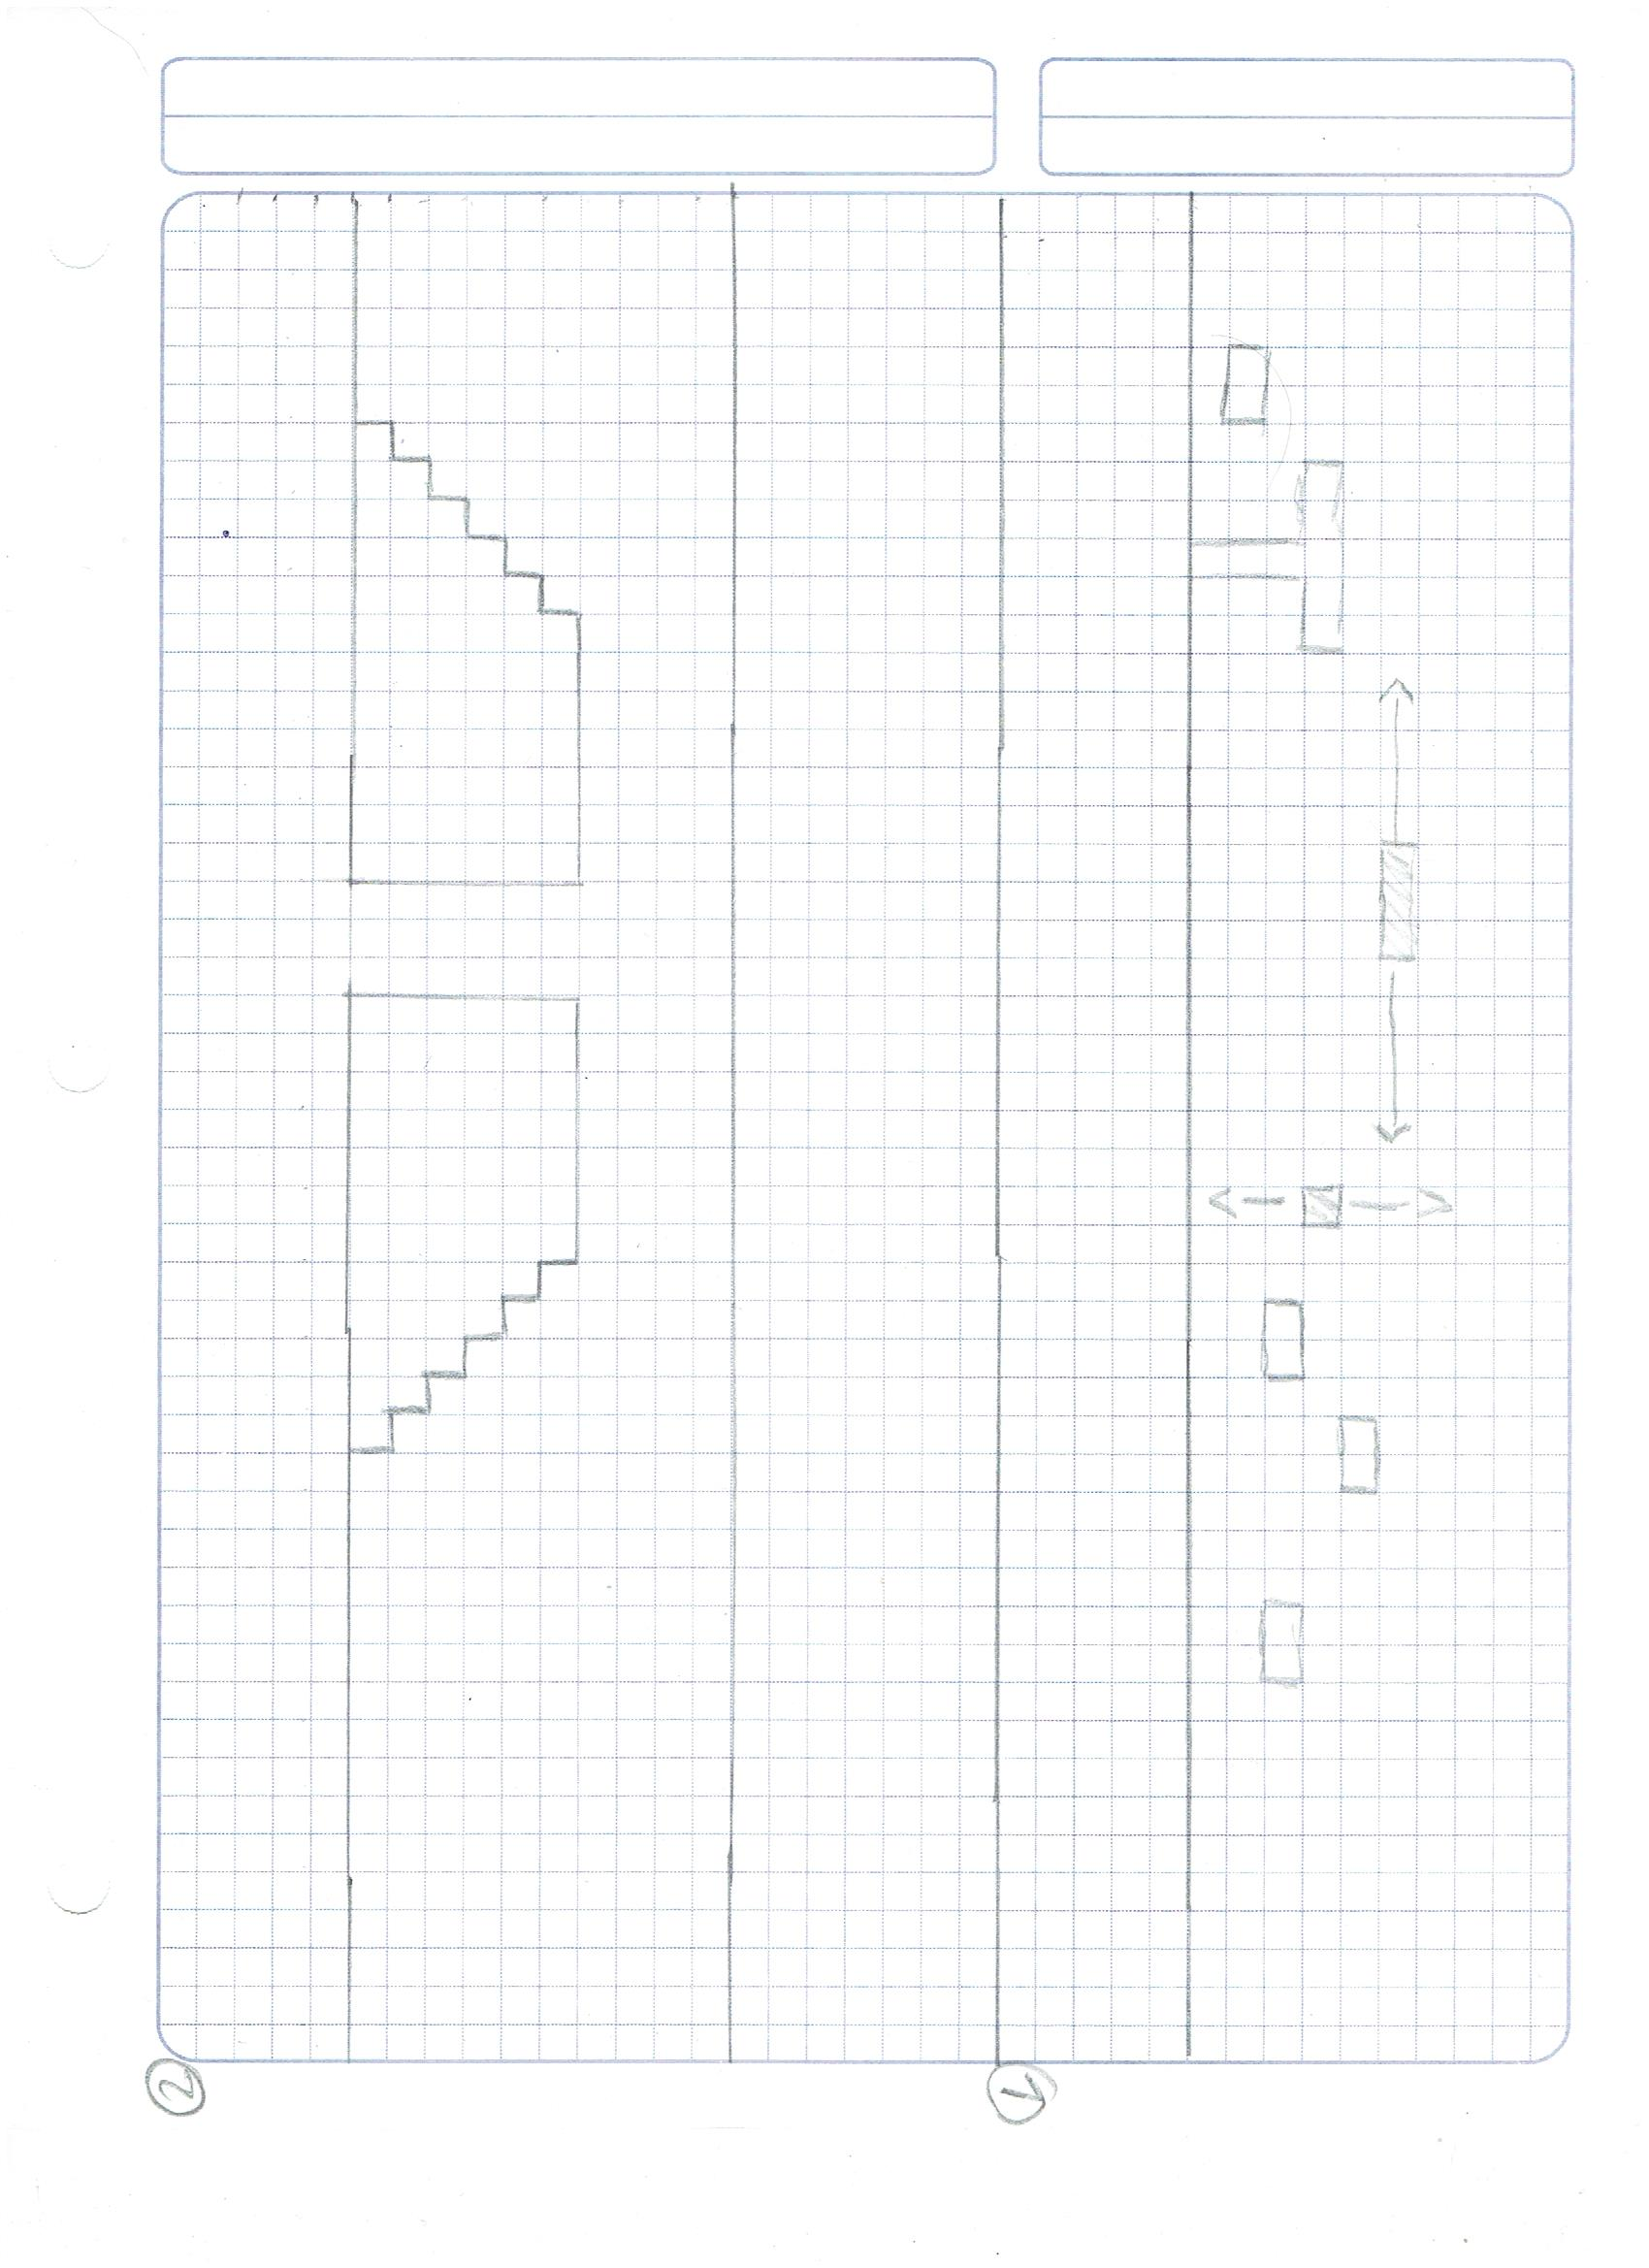
\includegraphics[width=5cm]{03TrabajoRealizado/DocProduccionR/imagenes/n7/11.jpeg}}
	\subfigure[Segunda parte del nivel]{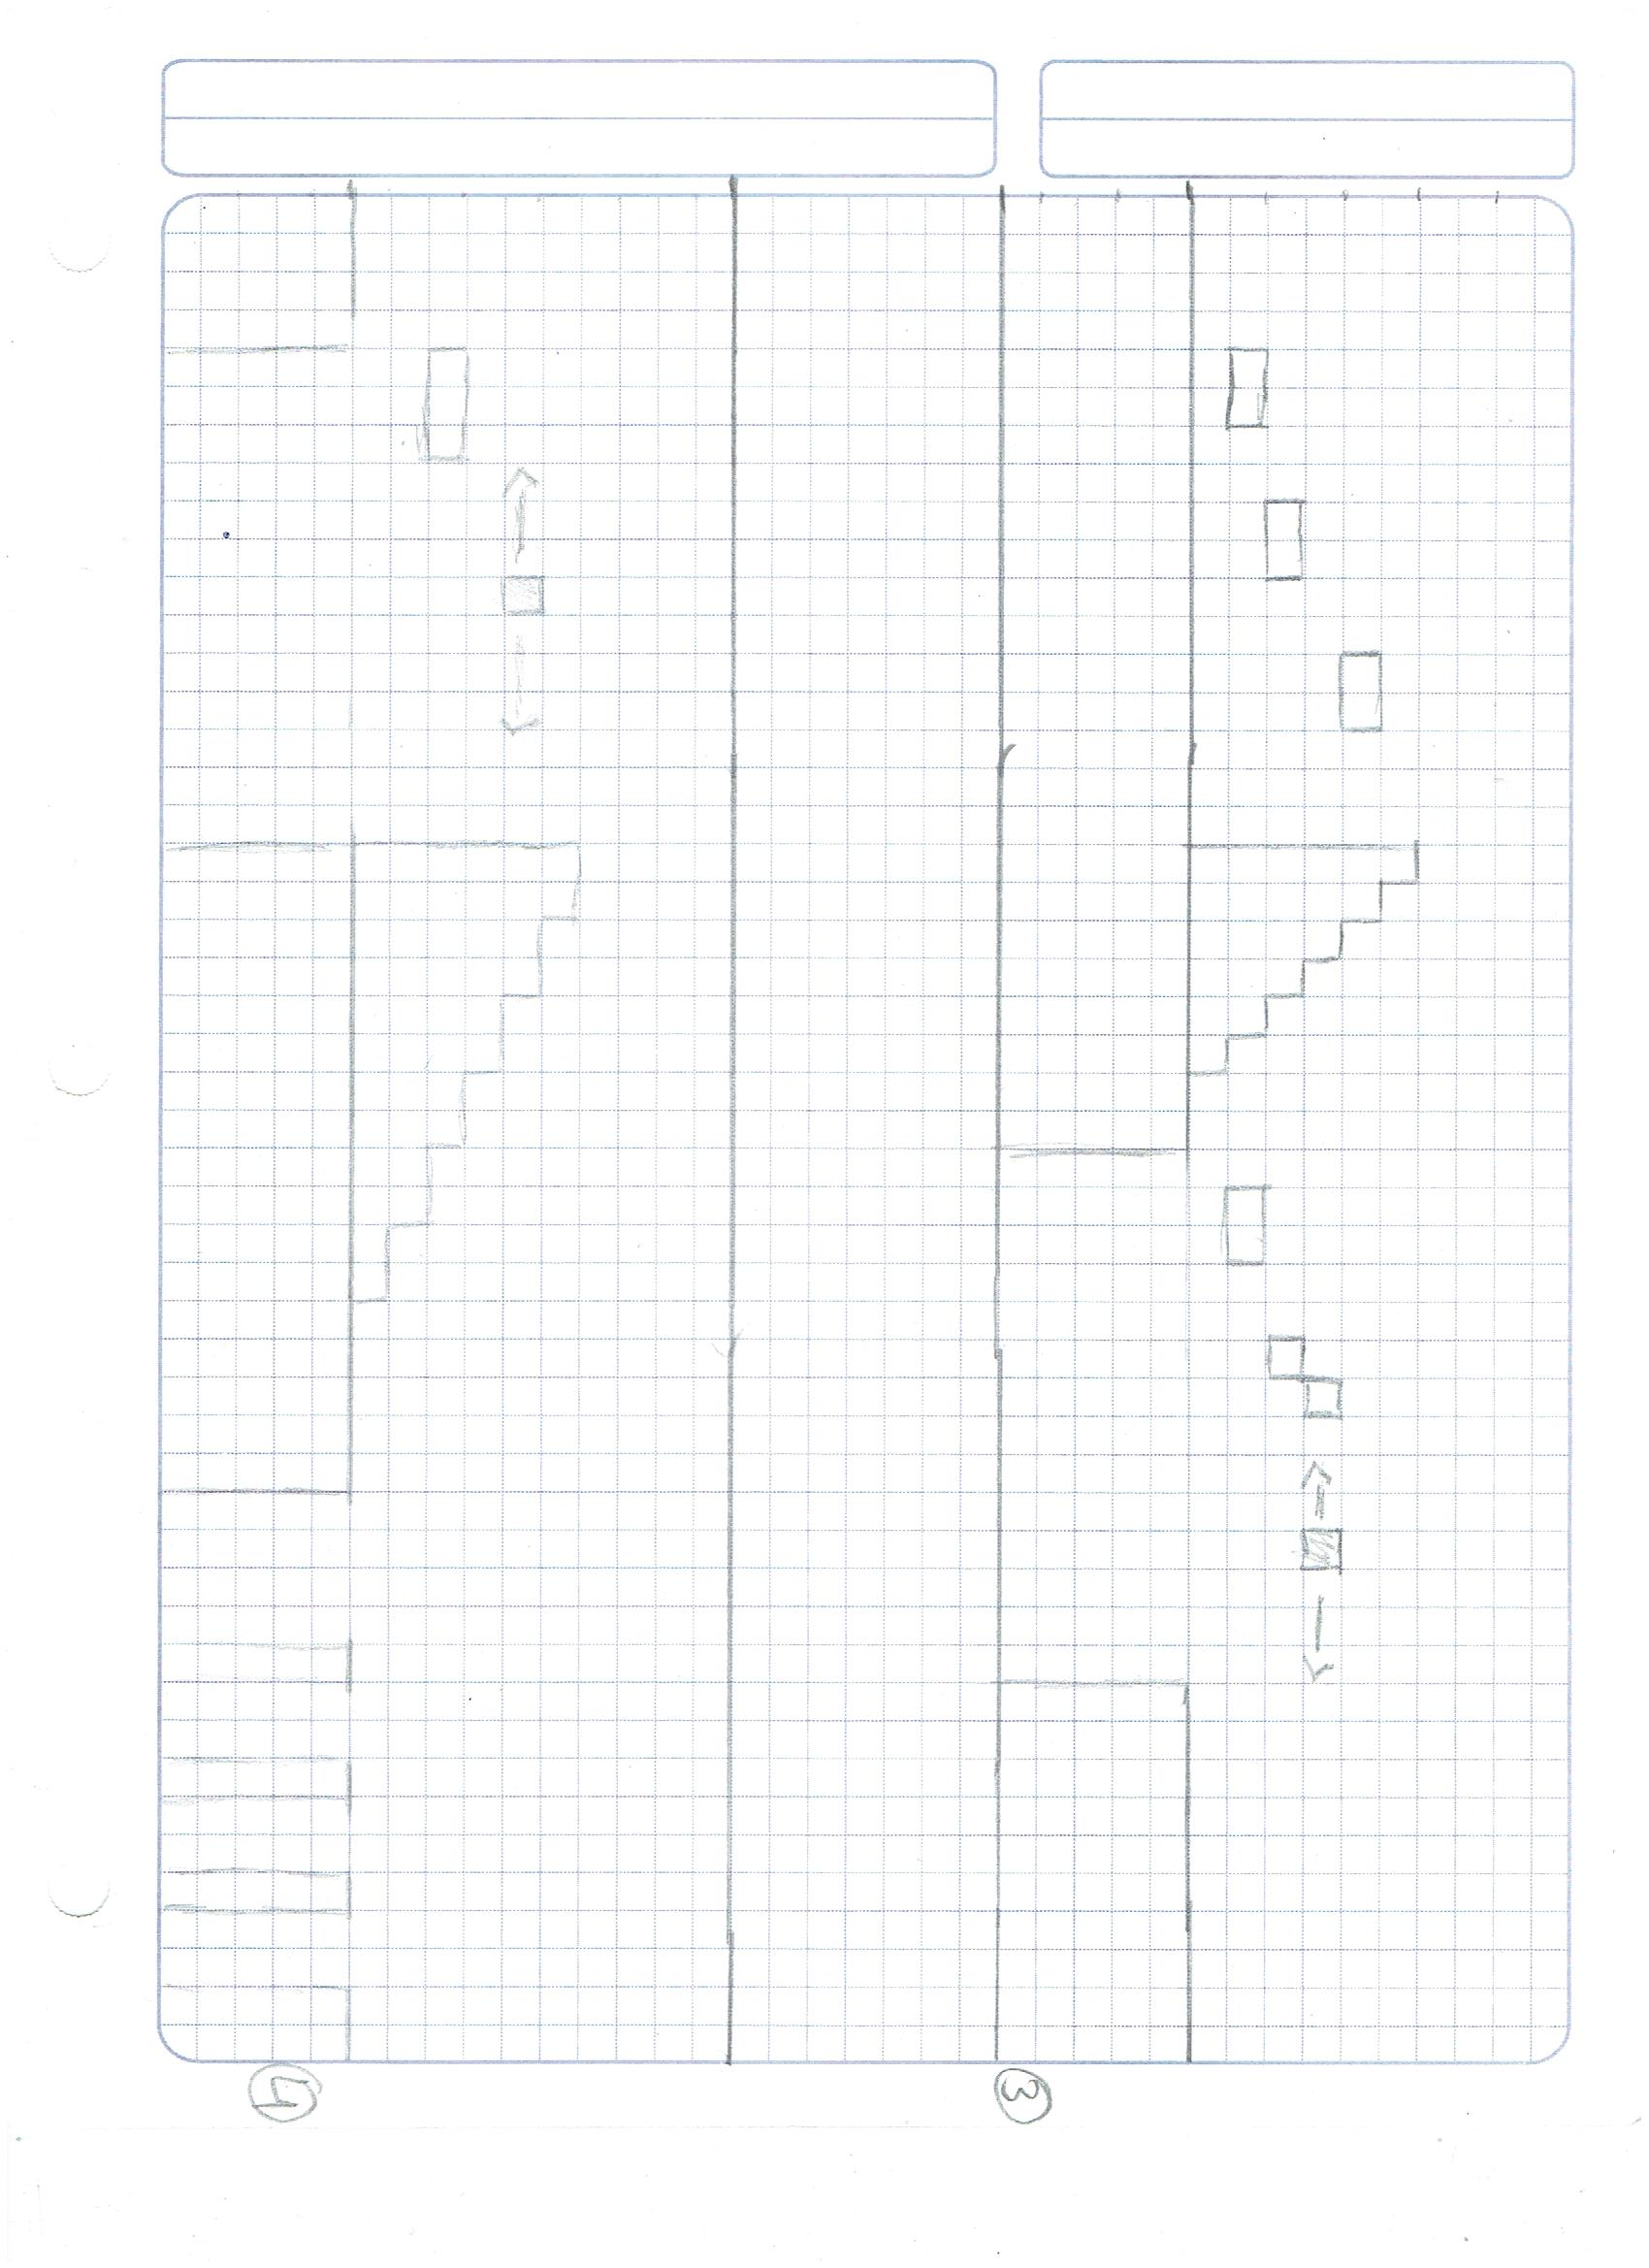
\includegraphics[width=5cm]{03TrabajoRealizado/DocProduccionR/imagenes/n7/12.jpeg}}
	\caption{Maquetado de nivel siete} \label{fig:n701}
\end{figure}  

Después se lleva la tarea de tomar todos los componentes solo de manera visual y adecuar el tamaño necesario, tomando en cuenta las medidas de los componentes anteriores. Dichas imágenes se pueden ver en la \ref{fig:n702}.
\begin{figure}[htbp]
	\centering
	\subfigure[Imagen jefe enemigo Itztlacoliuhqui.]{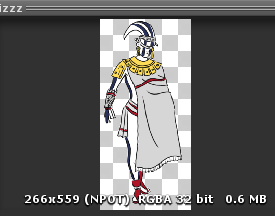
\includegraphics[width=5cm]{03TrabajoRealizado/DocProduccionR/imagenes/n7/n702.png}}
	\subfigure[Imagen de flecha de obsidiana.]{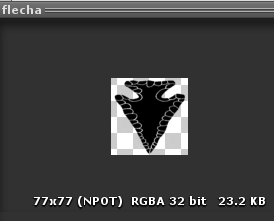
\includegraphics[width=5cm]{03TrabajoRealizado/DocProduccionR/imagenes/n7/n703.png}}
	\subfigure[Imagen de fuego.]{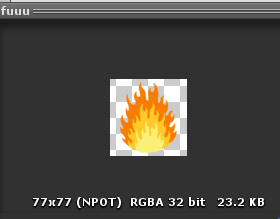
\includegraphics[width=5cm]{03TrabajoRealizado/DocProduccionR/imagenes/n7/n704.png}}
	\subfigure[Imagen de mano gigante.]{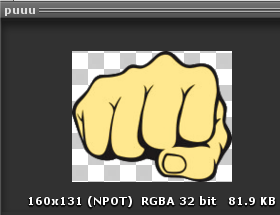
\includegraphics[width=5cm]{03TrabajoRealizado/DocProduccionR/imagenes/n7/n705.png}}
	\caption{Imágenes utilizadas para el nivel} \label{fig:n702}
\end{figure}

Después de reunir los componentes se da a la tarea de dar las acciones que realizarían descritas dentro de la figura \ref{fig:n703}. En esta parte se omitirá las plataformas con movimiento tanto horizontal como vertical, pues presentan el mismo comportamiento que los anteriores. También se omite los enemigos fantasmas mostrados en niveles anteriores. Dejando solo la interacción de una lluvia constante de flechas de obsidiana, para que el nivel no fuera sobre cargado, se determino que solo la lluvia se efectuara a una distancia horizontal del jugador a cierto tiempo y desapareciendo al choque con cualquier objeto por parte de la flecha.
\begin{figure}[htbp]
	\centering
	\subfigure[Caída constante de flechas de obsidiana a lo largo del nivel de plataforma.]{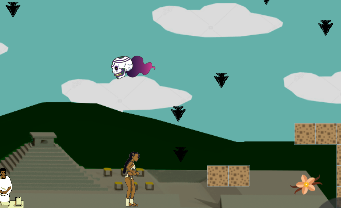
\includegraphics[width=5cm]{03TrabajoRealizado/DocProduccionR/imagenes/n7/n709.png}}
	\caption{Muestra de comportamiento de objetos} \label{fig:n703}
\end{figure}

Ya que se tiene los objetos con los comportamientos deseados se procede a ubicarlos según correspondan como se ve en la \ref{fig:n704}.
\begin{figure}
	\centering
	\caption{Maquetado llevado al motor de juego Unity.}
	\label{fig:n704}
	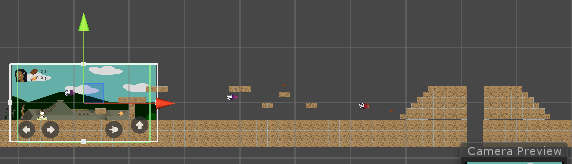
\includegraphics[width=0.5\textwidth]{03TrabajoRealizado/DocProduccionR/imagenes/n7/n701.png}
\end{figure}

Por último se establece las acciones que realiza el jefe enemigo Itztlacoliuhqui descritas en la siguiente figura \ref{fig:n705}.
\begin{figure}[htbp]
	\centering
	\subfigure[Caída aleatoria de forma horizontal de fuego sobre la superficie.]{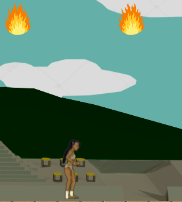
\includegraphics[width=5cm]{03TrabajoRealizado/DocProduccionR/imagenes/n7/n706.png}}
	\subfigure[Caída aleatoria de forma horizontal de una sola mano gigante sobre la superficie.]{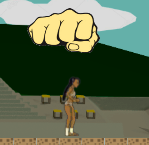
\includegraphics[width=5cm]{03TrabajoRealizado/DocProduccionR/imagenes/n7/n708.png}}
	\subfigure[Aparición de forma aleatoria horizontal de un numero determinado de flechas.]{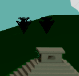
\includegraphics[width=5cm]{03TrabajoRealizado/DocProduccionR/imagenes/n7/n707.png}}
	\caption{Muestra de acciones de el jefe enemigo Itztlacoliuhqui. } \label{fig:n705}
\end{figure}

